\documentclass{../../fal_assignment}
\graphicspath{ {../../} }

\usepackage{enumitem}
\setlist{nosep} % Make enumerate / itemize lists more closely spaced
\usepackage[T1]{fontenc} % http://tex.stackexchange.com/a/17858
\usepackage{url}
\usepackage{todonotes}
\usepackage{float}

\title{Portfolio of Game Prototypes}
\author{Brian McDonald}
\module{GAM702}
\programme{MA Game Design}
\version{1.0}

\begin{document}

\maketitle

\section*{Introduction}

\begin{marginquote}
"It isn't enough to pick a path—you must go down it. By doing so, you see things you couldn't possibly see when you started out; you may not like what you see, some of it may be confusing, but at least you will have, as we like to say, 'explored the neighborhood.' The key point here is that even if you decide you're in the wrong place, there is still time to head toward the right place."
-- Ed Catmull, Creativity Inc.

\end{marginquote}
\marginpicture{flavour_pic}{
    \emph{Marvel's Spider-man: PS4}, early gameplay prototype showing web traversal mechanics.
}

For this assignment you will create \textbf{five} prototype games based on a series of provocations provided by the module tutor. In effect, you will be creating a small game prototype every two weeks. After the end of the two weeks, you will receive feedback from your Peers and the Module Tutors.

As a Game Designer it is up to you on what kind of game you create and what technology you will use to create the prototype. You can create a digital game, boardgame, cardgame, RPG Module or physical game. However, you will need to justify all your decisions in the Development Journal , see \textbf{Assignment 2}

For the final submission you have to select \textbf{three} prototypes that will go forward into your final summative submission.

\subsection*{Peer and self Assessment}
After each formative submission you will be required to play a selection of prototypes produced by your peer and even your own game. It is required that you engage with
this process through out the module. Every piece of feedback should be constructive and actionable, in addition, a portion of your mark will be derived on how you engage with this
feedback process. 

\subsection*{Assignment Setup} 

This assignment consists of \textbf{five formative submissions}, followed by a \textbf{single summative submission}.

After each formative submission you will receive feedback from your peers and module tutor. You should note this feedback and feed this into subsequent prototypes.  

The formative submissions consists of a single zip file, with the following folder structure. You can also find a template zip file on the Assignment Space in the Learning Space

\pagebreak
\subsection*{Digital Game Submission} 

\begin{figure}[H]
	\begin{center}
		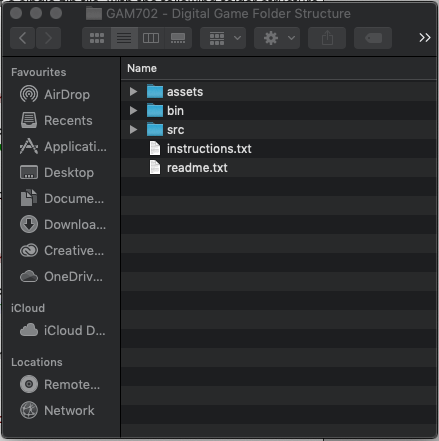
\includegraphics[height=0.4\textheight]{digital_games_folder_structure}
	\end{center}
	\caption{Recommended folder structure for formative submissions of Digital Games.}
	\label{fig:digital_game_folder_structure}
\end{figure}

\begin{itemize}
	\item The \textbf{instructions.txt} should contain any controls and other information required to play
	\item The \textbf{readme.txt} should contain a description of the game and any references to resources used for the game. These resources include assets, reference materials, tutorials etc
	\item The \textbf{src} folder should contain the project files and source code for the game
	\item The \textbf{bin} folder should contain project compiled executable
	\item The \textbf{assets} folder should contain all source assets used in the game including images, documents or text
\end{itemize}

\pagebreak
\pagebreak
\subsection*{Physical Game (including Boardgame, RPG and Folk Game)} 

\begin{figure}[H]
	\begin{center}
		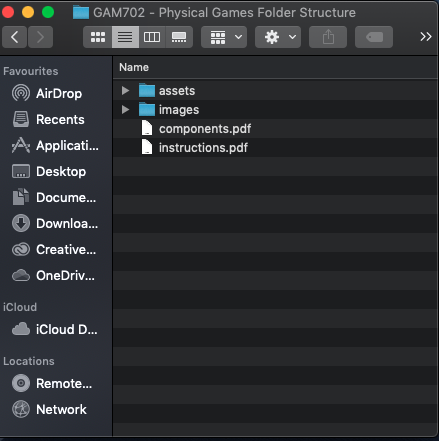
\includegraphics[height=0.4\textheight]{physical_games_folder_structure}
	\end{center}
	\caption{Recommended folder structure for formative submissions of Physical Games.}
	\label{fig:phyical_game_folder_structure}
\end{figure}

\begin{itemize}
	\item The \textbf{components.pdf} should contain a list of all components (dice, cubes, coins etc) required to play the game
	\item The \textbf{instructions.pdf} should be in the style of a board game manual, with setup instructions, a how to play guide and detailed rule instructions
	\item The \textbf{images} folder should contain images of the components, game setup and gameplay
	\item The \textbf{assets} folder should contain all source assets used in the game including images, documents or text
\end{itemize}

If you need a good example of rulebook layout please look at the following

\url{https://www.fairway3games.com/writing-rules-a-recipe/}
\url{https://www.orderofgamers.com/downloads/MansionsofMadness2ndEd_v1.pdf}

\pagebreak
\subsection*{Final Submission} 

\begin{figure}[H]
	\begin{center}
		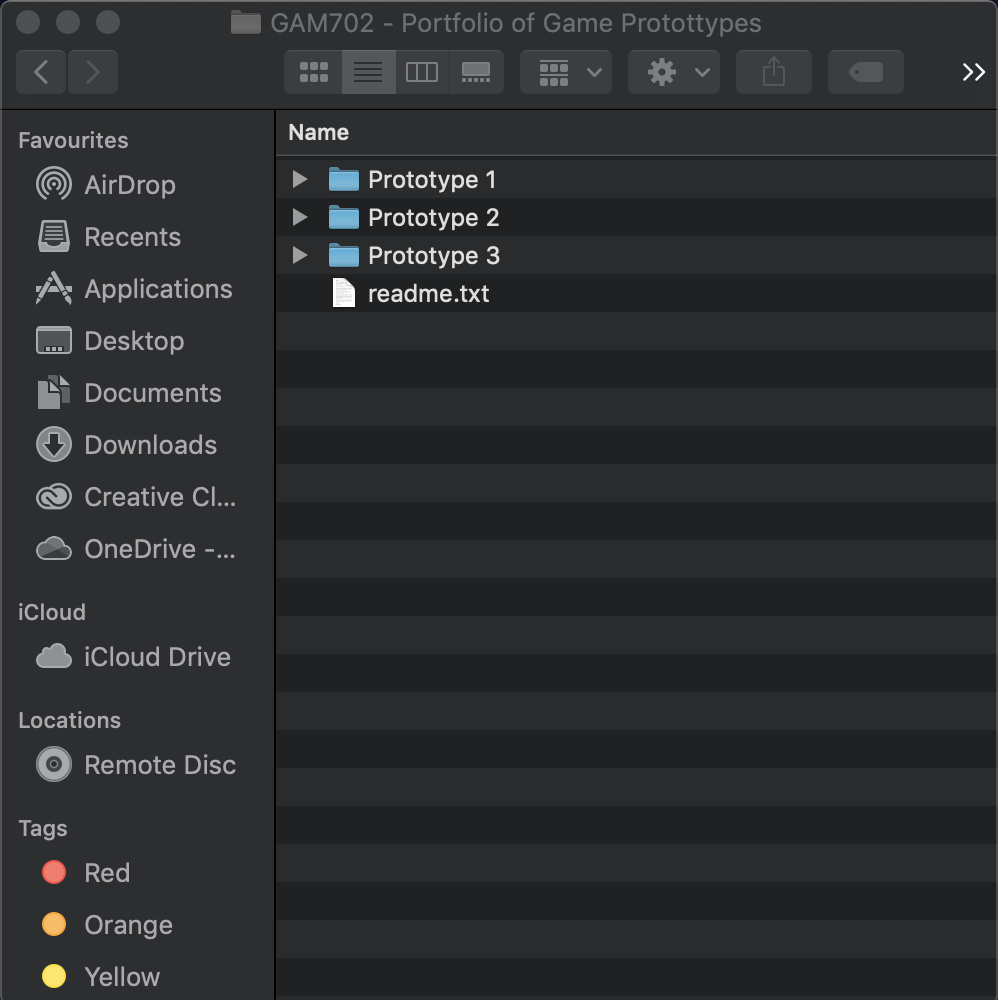
\includegraphics[height=0.4\textheight]{portfolio_folder_structure}
	\end{center}
	\caption{Recommended folder structure for final submission.}
	\label{fig:portfolio_folder_structure}
\end{figure}

At the end of the semester you will be required make a final summative submission of \textbf{three} of your \textbf{five} prototypes. 
Prepare a \textbf{single \texttt{.zip} file} containing your submissions \textbf{see folder structure}, and upload it to the appropriate submission area on LearningSpace.

\textbf{This final submission is subject to the usual university policies regarding late submission or non-submission,
as detailed in the course handbook ---
even if you have met all the formative deadlines,
failure to make a submission via LearningSpace by the summative deadline will be subject to penalties.}

\section*{Additional Guidance}



\section*{FAQ}

\begin{itemize}
	\item 	\textbf{What is the deadline for this assignment?} \\ 
    		Falmouth University policy states that summative deadlines must only be specified on the MyFalmouth system.
    		
	\item 	\textbf{What should I do to seek help?} \\ 
    		You can email your tutor for informal clarifications.  
    		
	\item 	\textbf{How will I receive feedback on my work?} \\ 
    		You will be given verbal feedback on your work during the session in which it is marked.
    		If you require more in-depth feedback or discussion, please book an appointment with your tutor.
    		
    	\item 	\textbf{Is this a mistake?} \\ 	
    		If you have discovered an issue with the brief itself, please inform the module tutor.
\end{itemize}

\rubrichead{All submissions and assessment criteria for this assignment are individual.}
\begin{markingrubric}
	%
	\firstcriterion{Basic Competency Threshold}{40\%}
	\gradespan{1}{\fail At least one part is missing or is inadequate.}
	\gradespan{5}{Adequate ability to generate ideas, problem solving, concepts and proposals in response to set briefs and/or self-initiated activity.
		\par The work demonstrates an adequate, ethically informed, real-world experience of industry/business environments and markets.
		\par Enough work is available to hold a meaningful discussion.
		\par Adequate participation in-class peer-review activities
		\par No breaches of academic integrity.}
	%
	\criterion{Appropriateness of tools and techniques}{15\%}
	\grade\fail 	No appropriate tools or techniques are used
	\par 		The tools selected through out the project have not matched the challenge of the briefs.
	\grade 		Only one tool/technique has been used throughout the project.
	\par 		The knowledge of this tool is fairly basic.  
	\grade 		Only one tool/technique has been used throughout the project.
	\par 		The knowledge of this tool has advanced throughout the project.
	\grade 		There has been a mix of two to three tools or techniques used. 
	\par 		The knowledge of these tools/techniques are fairly basic. 
	\par		The tools/techniques selected feel justified in terms of the game idea
	\grade 		There has been a mix of two to three tools or techniques used.
	\par 		The knowledge of this tool has advanced throughout the project.
	\par		The briefs have been satisfied.     
	\grade 		There has been a mix of two to three tools or techniques used
	\par		The knowledge exhibited of these tools are at near expert level
	\par		The briefs has been satisfied.
	%
	\criterion{Evolution of practice}{15\%}
	\grade\fail There has no evolution of practice.
	\par All games feel similar.
	\grade There is little evolution of practice.
	\par It feels like the designer hasn't properly learned from past prototypes.
	\grade This is some evolution of practice.
	\par There are some links in terms of lessons learned from previous projects.
	\grade There is much evolution of practice.
	\par There are visible direct links in terms of lessons learned from previous projects.
	\grade Considerable evolution of practice.
	\par Each prototype feels like a piece in a body of work.
	\grade Significant evolution of practice.
	\par There are clear lessons learned from each project.
	\par Each prototype feels like a piece in a body of work.
	%
	\criterion{Peer Assessment}{10\%}
	\grade\fail No engagement.
	\par The feedback was non existent or not useful at all
	\grade Little engagement.
	\par The feedback is not constructive or actionable.
	\grade Some engagement.
	\par The feedback is useful but doesn't go into enough detail to make any real impact.
	\grade Much engagement.
	\par The feedback has actionable points but requires more detail to be truly useful
	\grade Considerable engagement.
	\par The feedback is excellent, and contains many actionable points.
	\grade Significant engagement.
	\par The feedback is exemplary, it is actionable, contains alternative suggestions and approaches.
	%
	\criterion{Creativity of the Prototypes}{20\%}
	\grade\fail No creativity.
	\par The work is a clone of an existing work with mere cosmetic alterations.
	\grade Little creativity.
	\par The work is derivative of existing works, with only minor alterations.
	\grade Some creativity.
	\par The work is derivative of existing works, demonstrating little divergent and/or subversive thinking.
	\grade Much creativity.
	\par The work is somewhat novel, demonstrating some divergent and/or subversive thinking.
	\grade Considerable creativity.
	\par The work is novel, demonstrating significant divergent and/or subversive thinking.
	\grade Significant creativity.
	\par The work is highly original, with strong evidence of divergent and/or subversive thinking.
	%
	
\end{markingrubric}
\end{document}